\section{Js::String Class Reference}
\label{classJs_1_1String}\index{Js::String@{Js::String}}
{\tt \#include $<$string.h$>$}

Inheritance diagram for Js::String::\begin{figure}[H]
\begin{center}
\leavevmode
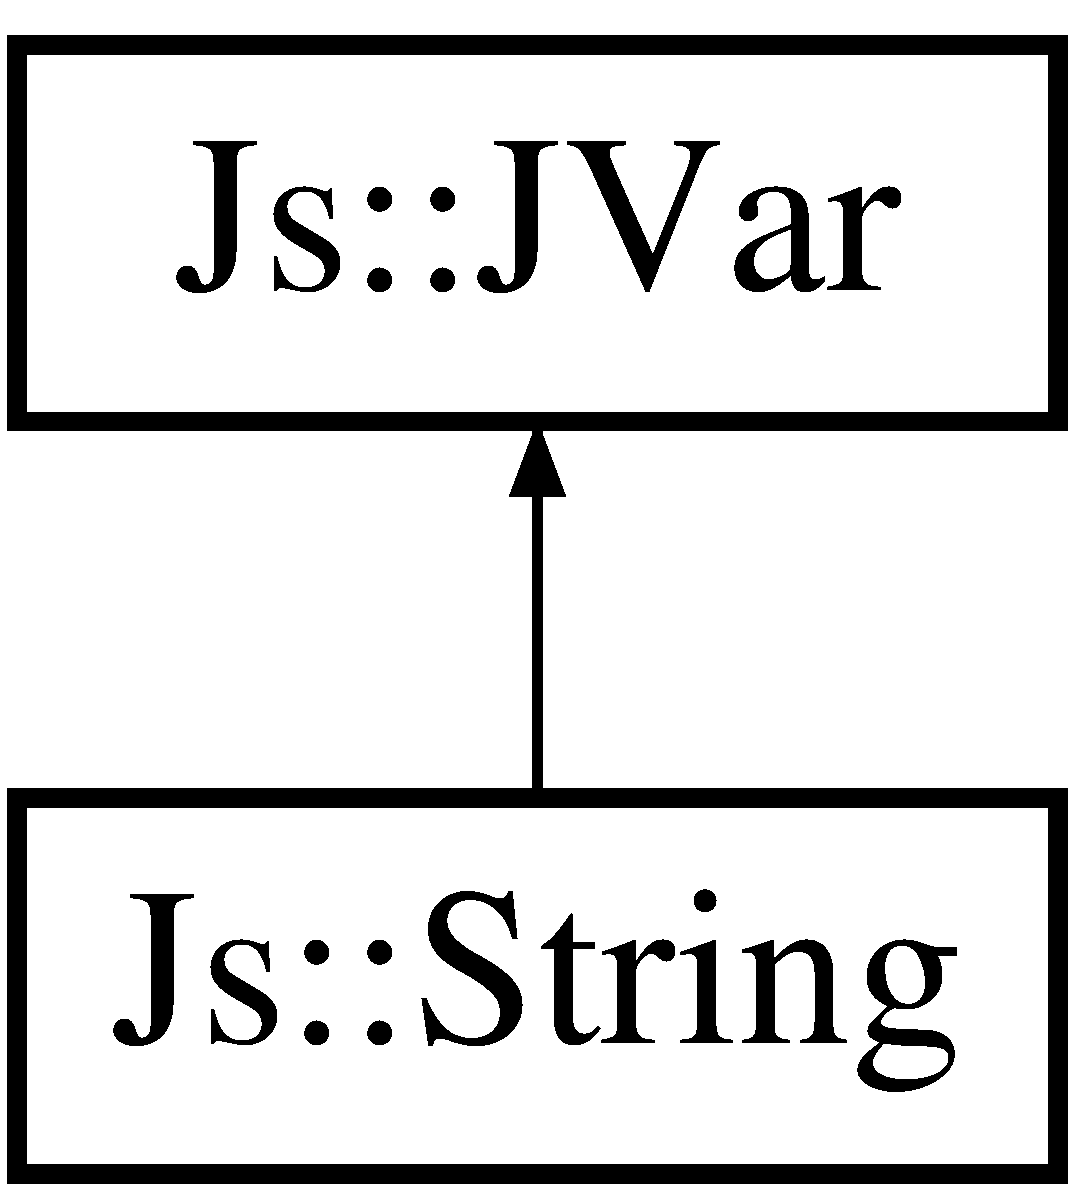
\includegraphics[height=2cm]{classJs_1_1String}
\end{center}
\end{figure}


\subsection{Detailed Description}
\begin{Desc}
\item[Author:]Neel Basu $<$neel$>$ \end{Desc}


The documentation for this class was generated from the following files:\begin{CompactItemize}
\item 
string.h\item 
string.cpp\end{CompactItemize}
